\input{../templates/course_definitions}
% This Document contains the information about this course.

% Authors of the slides
\author{Tobias Hanf, Manik Khurana}

% Name of the Course
\institute{Java-Course}

% Fancy Logo
\titlegraphic{\hfill\includegraphics[height=1.25cm]{../templates/fsr_logo_cropped}}


\title{Java}
\subtitle{Inheritance}
\date{\today}

\begin{document}

\begin{frame}
	\titlepage
\end{frame}
\begin{frame}{Overview}
	\setbeamertemplate{section in toc}[sections numbered]
	\tableofcontents
\end{frame}



\section{Arrays}
\begin{frame}[fragile]{Array}
	An array is a data-type that can hold a \textbf{fixed number} of elements. 
	An Element can be any simple data-type or object.
	\begin{lstlisting}
	public static void main(String[] args) {
	
	    int[] intArray = new int[10];
	    intArray[8] = 7; // assign 7 to the 9th element
	    intArray[9] = 8; // assign 8 to the last element
	    
	    System.out.println(intArray[8]); // prints: 7
	}
	\end{lstlisting}
	You can access every element via an index. A n-element array has indexes from 0 to (n-1).
\end{frame}

\begin{frame}[fragile]{Array Initialization} % AE
	You can initialize an array with a set of elements.
	\begin{lstlisting}
	public static void main(String[] args) {
	
	    int[] intArray = {3, 2, 7};
	    
	    System.out.println(intArray[0]); // prints: 3
	    System.out.println(intArray[1]); // prints: 2
	    System.out.println(intArray[2]); // prints: 7
	}
	\end{lstlisting}
\end{frame}

\begin{frame}[fragile]{Alternative Declaration}
	There two possible positions for the square brackets. 
	%I would recommend the first version to improve readability.
	\begin{lstlisting}
	public static void main(String[] args) {

	    // version 1	
	    int[] intArray1 = new int[10];
	    
	    // version 2
	    int intArray2[] = new int[10];
	}
	\end{lstlisting}
\end{frame}

\subsection{Multi-Dimensional Array}
\begin{frame}[fragile]{2-Dimensional Array}
	Arrays work with more than one dimension. 
	An m-dimensional array has m indexes for one element.
	\begin{lstlisting}
	public static void main(String[] args) {

	    // an array with 100 elements
	    int[][] intArray = new int[10][10];
	    
	    intArray[0][0] = 0;
	    intArray[0][9] = 9;
	    intArray[9][9] = 99;
	}
	\end{lstlisting}
\end{frame}

\begin{frame}[fragile]{Assignment with Loops}
	Loops are often used to assign elements in arrays.
	\begin{lstlisting}
	public static void main(String[] args) {

	    int[][] intArray = new int[10][10];
	    
	    for(int i = 0; i < 10; i++) {
	        for(int j = 0; j < 10; j++) {
	            intArray[i][j] = i*10 + j;
	        }
	    }
	}
	\end{lstlisting}
\end{frame}

\begin{frame}[fragile]{Arrays with objects}
	Loops are often used to assign elements in arrays.
	\begin{lstlisting}
	public static void main(String[] args) {

	    Student[][] studentArray = new Student[10][10];
	    
	    for(int i = 0; i < 10; i++) {
	        for(int j = 0; j < 10; j++) {
	            intArray[i][j] = new Student();
	        }
	    }
	}
	\end{lstlisting}
\end{frame}

\section{Inheritance}
\subsection{Inheritance}

\begin{frame}{Example}
	A school has students and teacher.\\
	Every student has the following attributes:
	\begin{itemize}
		\item name
		\item age
		\item email
		\item lessons
		\item Name of his class
	\end{itemize}
	Every teacher has the following attributes:
	\begin{itemize}
		\item name
		\item age
		\item email
		\item subjects
		\item salary
		\item hours
	\end{itemize}
\end{frame}

\begin{frame}{Creating Inheritance}
	They have the same subset of attributes:
	\begin{itemize}
		\item name
		\item age
		\item email
	\end{itemize}
	Why not define these attributes somewhere else and say these are part of a student and teacher?
\end{frame}

\begin{frame}{What is inheritance?}
	This is inheritance.
	\begin{itemize}
		\item basing an object or class upon another object or class
		\item creates an hierarchy of classes
		\item classes on top of the hierarchy are the \textbf{superclasses}
		\item classes below a \textbf{superclass} are called \textbf{subclasses}
		\item objects create from \textbf{superclasses} are called \textbf{parent objects}
		\item objects create from \textbf{subclasses} are called \textbf{child objects}
	\end{itemize}
\end{frame}

\begin{frame}{UML class diagram}
	\begin{center}
		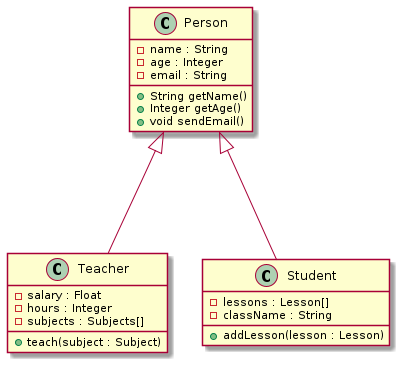
\includegraphics[height=.8\textheight]{04-inheritance/student_teacher.png}
	\end{center}	
\end{frame}

\begin{frame}{Student class}
	\begin{center}
		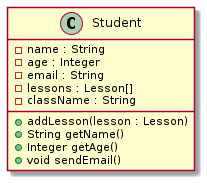
\includegraphics[height=.8\textheight]{04-inheritance/student.png}
	\end{center}	
\end{frame}


\begin{frame}[fragile]{A special Person}
	Our class \emph{Student} is a kind of \emph{Person} denoted by the keyword \textbf{extends}.
	\begin{itemize}
		\item \emph{Student} is a \textbf{subclass} of the class \emph{Person}
		\item \emph{Person} is the \textbf{superclass} of the class \emph{Student}
	\end{itemize}
	\begin{lstlisting}
	public class Student extends Person {
	
	}
	\end{lstlisting}
	\vfill
	As mentioned implicitly above a class can has multiple subclasses. 
	But a class can only inherit directly from one superclass.
\end{frame}

\begin{frame}[fragile]{Example}
	We have the classes: \emph{School}, \emph{Person} and \emph{Student}.
	They will be used for every example in this section and they will grow over time.
	\begin{lstlisting}
	public class Person {
	
	    private String name;
	    private int age;
	    private String email
	    
    
	    public void setEmail(String email) {
	    	this.email = email;    
	    }
    
    	public void sendEmail(String message){
    		System.out.println("To: " this.email 
    							+ " \n" + message);
    	}
	}
	\end{lstlisting}
\end{frame}

\begin{frame}[fragile]{Inherited Methods}
	The class \emph{Student} also inherits all methods from the superclass \emph{Person}.
	\begin{lstlisting}
	public class School {
	
	    public static void main(String[] args) {
	    
	        Student Student = new Student();
	        
	        Student.setEmail("john@school.org");
	        
	        Student.sendEmail("Hello");
	        
	        // prints: 	To: john@school.org
	        //			Hello
	    }	
	}
	\end{lstlisting}
\end{frame}

\begin{frame}[fragile]{Override Methods}
	The method sendEmail() is now additional definded in \emph{Student}.
	\begin{lstlisting}[escapechar=!]
	public class Student extends Person {
	
	    @Override
	    public void sendEmail(String message){
	    	System.out.println("To: " this.email + " \n" +
	    				"Dear student :" + message);
    	}	
	}
	\end{lstlisting}
	% programer is AE
	\texttt{@Override} is an annotation. 
	It helps the programer to identify overwritten methods.
	It is not neccessary for running the code but improves readability.
	What annotations else can do we discuss in a future lesson.
\end{frame}
\begin{frame}[fragile]{Override Methods}
	Now the method \texttt{sendEmail()} defined in \emph{Student} will be used instead of the method defined
	in the superclass \emph{Person}.
	\begin{lstlisting}
	public class School {
	
	    public static void main(String[] args) {
	    
	        Student Student = new Student();
	        
	        Student.setEmail("john@school.org");
	        
	        Student.sendEmail("Hello");
	        // prints: 	To: john@school.org
	        //			Dear student: Hello
	    }	
	}
	\end{lstlisting}
\end{frame}

\subsection{Constructor}
\begin{frame}[fragile]{Super()}
	If we define a \textbf{constructor with arguments} in \emph{Person} we have to define a constructor
	with the same list of arguments in every subclass.
	\begin{lstlisting}[basicstyle=\ttfamily\scriptsize]
	public class Person {
	
	    private String name;
	    private int age;
	    private String email;
	    
	    public Person(String name, int age, String email) {
	        this.name = name;
	        this.age = age;
	        this.email = email;
	    }
	    	    
	    public void sendEmail(String message){
	    	System.out.println("To: " this.email 
	    	+ " \n" + message);
	    }
	}
	\end{lstlisting}
\end{frame}

\begin{frame}[fragile]{Super()}
	For the constructor in the subclass \emph{Student} we can use \texttt{super()} to call the constructor
	from the superclass.
	\begin{lstlisting}[escapechar=!]
	public class Student extends Person {

	    public Student(String name, int age, String email) {
	    	super(name, age, email);
	    }
	
	    @Override
	    public void sendEmail(String message){
	    	System.out.println("To: " this.email + " \n" +
	    	"Dear student :" + message);
	    }	
	}
	\end{lstlisting}
\end{frame}

\begin{frame}[fragile]{Super() - Test}
	\begin{lstlisting}
	public class School {
	    
	    public static void main(String[] args) {	    
	        Student Student = 
	            new Student("John", 16, "john@school.org");
	        
	        Student.sendEmail("Hello");
	        // prints: 	To: john@school.org
	        //			Dear student: Hello
	    }
	}
	\end{lstlisting}
\end{frame}

\subsection{Implicit Inheritance}
\begin{frame}{Object}
	Every class is a subclass from the class \emph{Object}. 
	Therefore every class inherits methods from \emph{Object}.
	\vfill
	See \scriptsize\url{http://docs.oracle.com/javase/7/docs/api/java/lang/Object.html} \normalsize for
	a full reference of the class \emph{Object}.
\end{frame}

\begin{frame}[fragile]{toString()}
	\emph{Student} is a subclass of \emph{Object}.
	Therefore \emph{Student} inherits the method \texttt{toString()} from \emph{Object}.\\
	\texttt{System.out.println(argument)} will call \texttt{argument.toString()} to receive
	a printable String.
	\begin{lstlisting}[escapechar=!]
	public class School {
	    
	    public static void main(String[] args) {	    
	        Student Student = 
	            new Student("John", 16, "john@school.org");
	        
	        System.out.println(Student);
	        // prints: Student@_some_HEX-value_
	        // for example: Student@4536ad4d
	    }
	}
	\end{lstlisting}
\end{frame}

\begin{frame}[fragile]{Override toString()}
	\begin{lstlisting}[escapechar=!]
	public class Student extends Person {

	    public Student(String name, int age, String email) {
	    	super(name, age, email);
	    }
	
	    @Override
	    public String toString() {
	        return "Student: " +  this.name;
	    }	
	}
	\end{lstlisting}
\end{frame}

\begin{frame}[fragile]{Override toString() - Test}
	\begin{lstlisting}
	public class School {
	    
	    public static void main(String[] args) {	    
	        Student Student = 
	            new Student("John", 16, "john@school.org");
	        
	        System.out.println(Student);
	        // Student: John
	    }
	}
	\end{lstlisting}
\end{frame}

\section{Programming}
\begin{frame}
	\begin{center}
		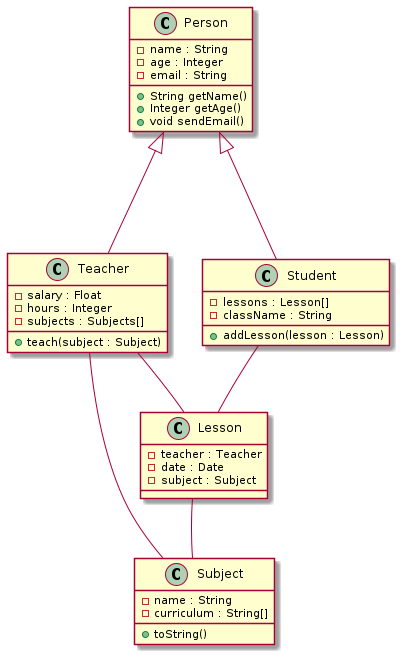
\includegraphics[height=\textheight]{04-inheritance/student_teacher_lesson.png}
	\end{center}

\end{frame}


\end{document}